\documentclass{article} % For LaTeX2e
\usepackage{nips15submit_e,times}
\usepackage{hyperref}
\usepackage{url}
\usepackage{caption}
\usepackage{refstyle}
\usepackage{amsmath}
\usepackage{times}
\usepackage{epsfig}
\usepackage{graphicx}
\usepackage{amsmath}
\usepackage{amssymb}
\usepackage{algpseudocode}
\usepackage{algorithm}
%\usepackage{subcaption}
\usepackage{subfig}
\usepackage{listings}
\usepackage{tabu}
\usepackage{float}
\IfFileExists{xxx_inclu}{\newcommand{\fix}{\marginpar{FIX}}
\newcommand{\new}{\marginpar{NEW}}
\renewcommand*{\thesubfigure}{\arabic{subfigure}}
\usepackage{caption}
\usepackage{refstyle}
%\usepackage{amsmath}
\usepackage{times}
\usepackage{epsfig}
%\usepackage{amsmath}
\usepackage{amssymb}}{.}
\restylefloat{table}
%\documentstyle[nips14submit_09,times,art10]{article} % For LaTeX 2.09

\title{CSE 253 PA3. Deep Convolutional Network for Image Classification and Transfer Learning}


\author{
Siwei Guo \\
Department of Electrical and\\ 
Computer Engineering\\
University of California San Diego\\
San Diego, CA 92037 \\
\texttt{s9guo@eng.ucsd.edu} \\
\And
Jingyi Yang \\
Department of Electrical and\\ 
Computer Engineering\\
University of California San Diego\\
San Diego, CA 92037 \\
\texttt{jiy349@eng.ucsd.edu} \\
\And
Meng Yue \\
Department of Electrical and\\ 
Computer Engineering\\
University of California San Diego\\
San Diego, CA 92037 \\
\texttt{yum107@eng.ucsd.edu} \\
\And
WenXin Ling \\
Department of \\
Computer Science Engineering\\
University of California San Diego\\
San Diego, CA 92037 \\
\texttt{wxling@eng.ucsd.edu} \\
}
\graphicspath{fig/}
% The \author macro works with any number of authors. There are two commands
% used to separate the names and addresses of multiple authors: \And and \AND.
%
% Using \And between authors leaves it to \LaTeX{} to determine where to break
% the lines. Using \AND forces a linebreak at that point. So, if \LaTeX{}
% puts 3 of 4 authors names on the first line, and the last on the second
% line, try using \AND instead of \And before the third author name.

\nipsfinalcopy % Uncomment for camera-ready version

\begin{document}


\maketitle

\begin{abstract}
Convolutional Neural Networks have been applied to visual tasks since the late 1980s, but were not popular until the mid-2000s when developments in computing power and the advent of large amounts of labeled data contributed to advancement. By comparing different models of CNN, AlexNet, GoogLeNet and a self-built one, GoogLeNet reports to have the highest accuracy of 99.2\%, AlexNet 98.5\%, and the self-build one 97.4\%.
\IfFileExists{xxx_abstr}{We also applied transfer learning on a small dataset and achieved an accuracy of 75.54\%. In addition, we did visualization to illustrate what role each CNN block plays, and also designed feature extraction experiment to show the importance of the depth of the neural network to the classification performance.}{.}
\end{abstract}

\section{Introduction}
Deep learning models have achieved remarkable results in image classification problems. This approach is more efficient and give much better result compare to traditional modelling approach. However, the learning process of Neural Network is not comprehensible compare to traditional method. Therefore, in this work, we trained three different CNN models on CIFAR-10 Dataset. First, we build a simple 6 layer shallow neural network. Then, we tried some other existing sucessful network models, AlexNet and GoogLeNet. We experiented different parameters, such as kernel size, different layers and other techniques.

\IfFileExists{xxx_intro}{Transfer learning is the method of reusing trained models on different tasks. Convolutional networks learn their features. Thus by training deep convolutional networks on large-scale datasets, we can train features that can be applied to other datasets. We apply a trained deep network to a relatively smaller dataset, retrain the classification layers and show the effectiveness of such approach.

In CNN model trained for image classification, the first convolution layer basically picks simple, local geometry features from input images(corners, lines, sketches), whereas higher-level convolution layers tend to extract semantic informations in wider receptive field(objects components). We visualized the first convolution layer and last convolution layer outputs, also the filter weights from the first convolution layer. This also implies depth of the neural network plays an important part in image classfication problem. Hence we designed feature extraction experiment in the last to show the significant degeneracy of classification ability after removing last several convolutional blocks of a classical CNN model VGG16.}{.}

\section{Deep CNN for Image Classification}
Using images from CIFAR-10 Dataset, we used three architectures to test a CNN's accuracy vs the number of 
epochs. Specifically, we built an AlexNet with , partial GoogLeNet with 18 convolutions, and a self-built 
net with . Generally, the comparision between AlexNet and self-build network indicates how the depth of 
network influence the performance. The comparision between AlexNet and GoogLeNet shows how difference architecture
perform differently and Inception model's ability to speed up training process. We also tried different
parameters on self-build model to test maxpooling, kernel size, Xavier initialization and batch normalization. 



\subsection{AlexNet Model}
The first model we built was an AlexNet model. AlexNet has been proved to be a break through in the
field of deep learning and can achieve good performance. Follow the rule of "don't be a hero", we
first borrowed Alex Krizhevsky's model. We built an AlexNet with 5 convolutions and 3 fully connected
 layers and the diagram is show in \figref{alex} (right). The kernel size for each convolution 
 is 5, 5, 3, 3, 3 with batch normalization, Xavier initialization and Adam Optimizer. The accuracy 
 plot is also shown in \figref{alex} (left). For AlexNet, we reduced the size of convolution kernel 
 from 11x11 to 5x5 since our image size is relatively small. 11x11 kernel will take over 1/3 of the 
 image pixel and return a more global features instead of local features that we want. It also turns 
 out that 5x5 works better compare to 11x11 kernel in terms of both training speed and accuracy.

\begin{figure}[h]
    \centering
    \subfloat[Accuracy vs. Epoch]{{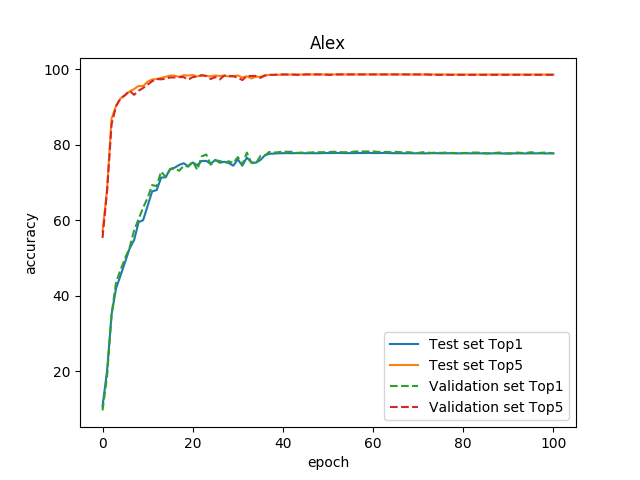
\includegraphics[width=6cm]{alexnet.png} }}
    \qquad
    \subfloat[Alex Net Diagram]{{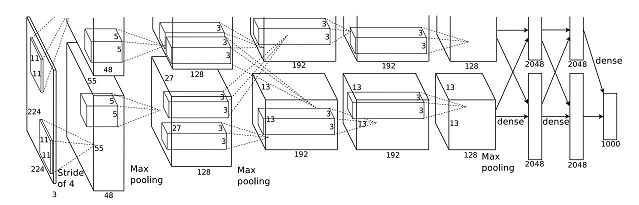
\includegraphics[width=6cm]{alexdiag.png} }}
    \caption{AlexNet Model}
    \label{fig:alex}
\end{figure}
 
 \subsection{Self-built Model}
 We also tried building a self-built architecture with 3 convolutions and 3 fully connected layers, 
 with kernel size 3, 3, 3 as shown in \figref{self}. We added max pooling into self-build architecture since max pooling can 
 downsize the feature map and introduce some amount of translation invariance to the network. 
 Then we also add batch normalization after each layer since batch normalization can both speed up
 the training process by removing the covariance shift and force the mean of weight to be zero.
 Batch normalization is done by calculating z-score 
 \begin{equation}
     \hat{x}_k = \frac{x_k-\mu_k}{\sqrt{\sigma_k+\epsilon}}
 \end{equation} where $\mu_k$ and $\sigma_k$ are the mean and variance of minibatch.\
 \begin{figure}[h]
    \centering
    \subfloat[Accuracy vs. Epoch]{{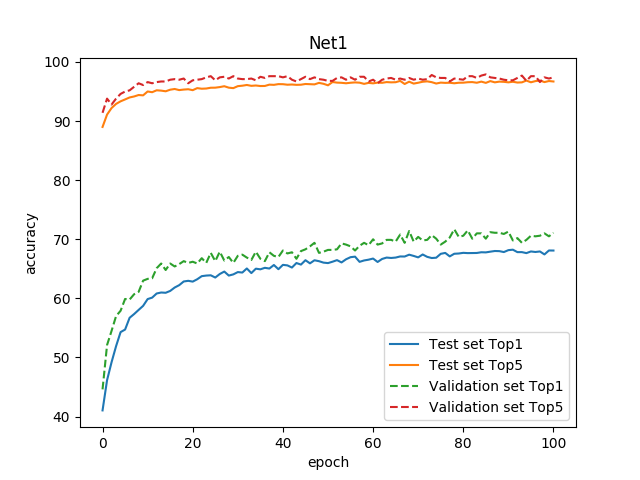
\includegraphics[width=6cm]{selfnet.png} }}
    \qquad
    \subfloat[Self-built Net Diagram]{{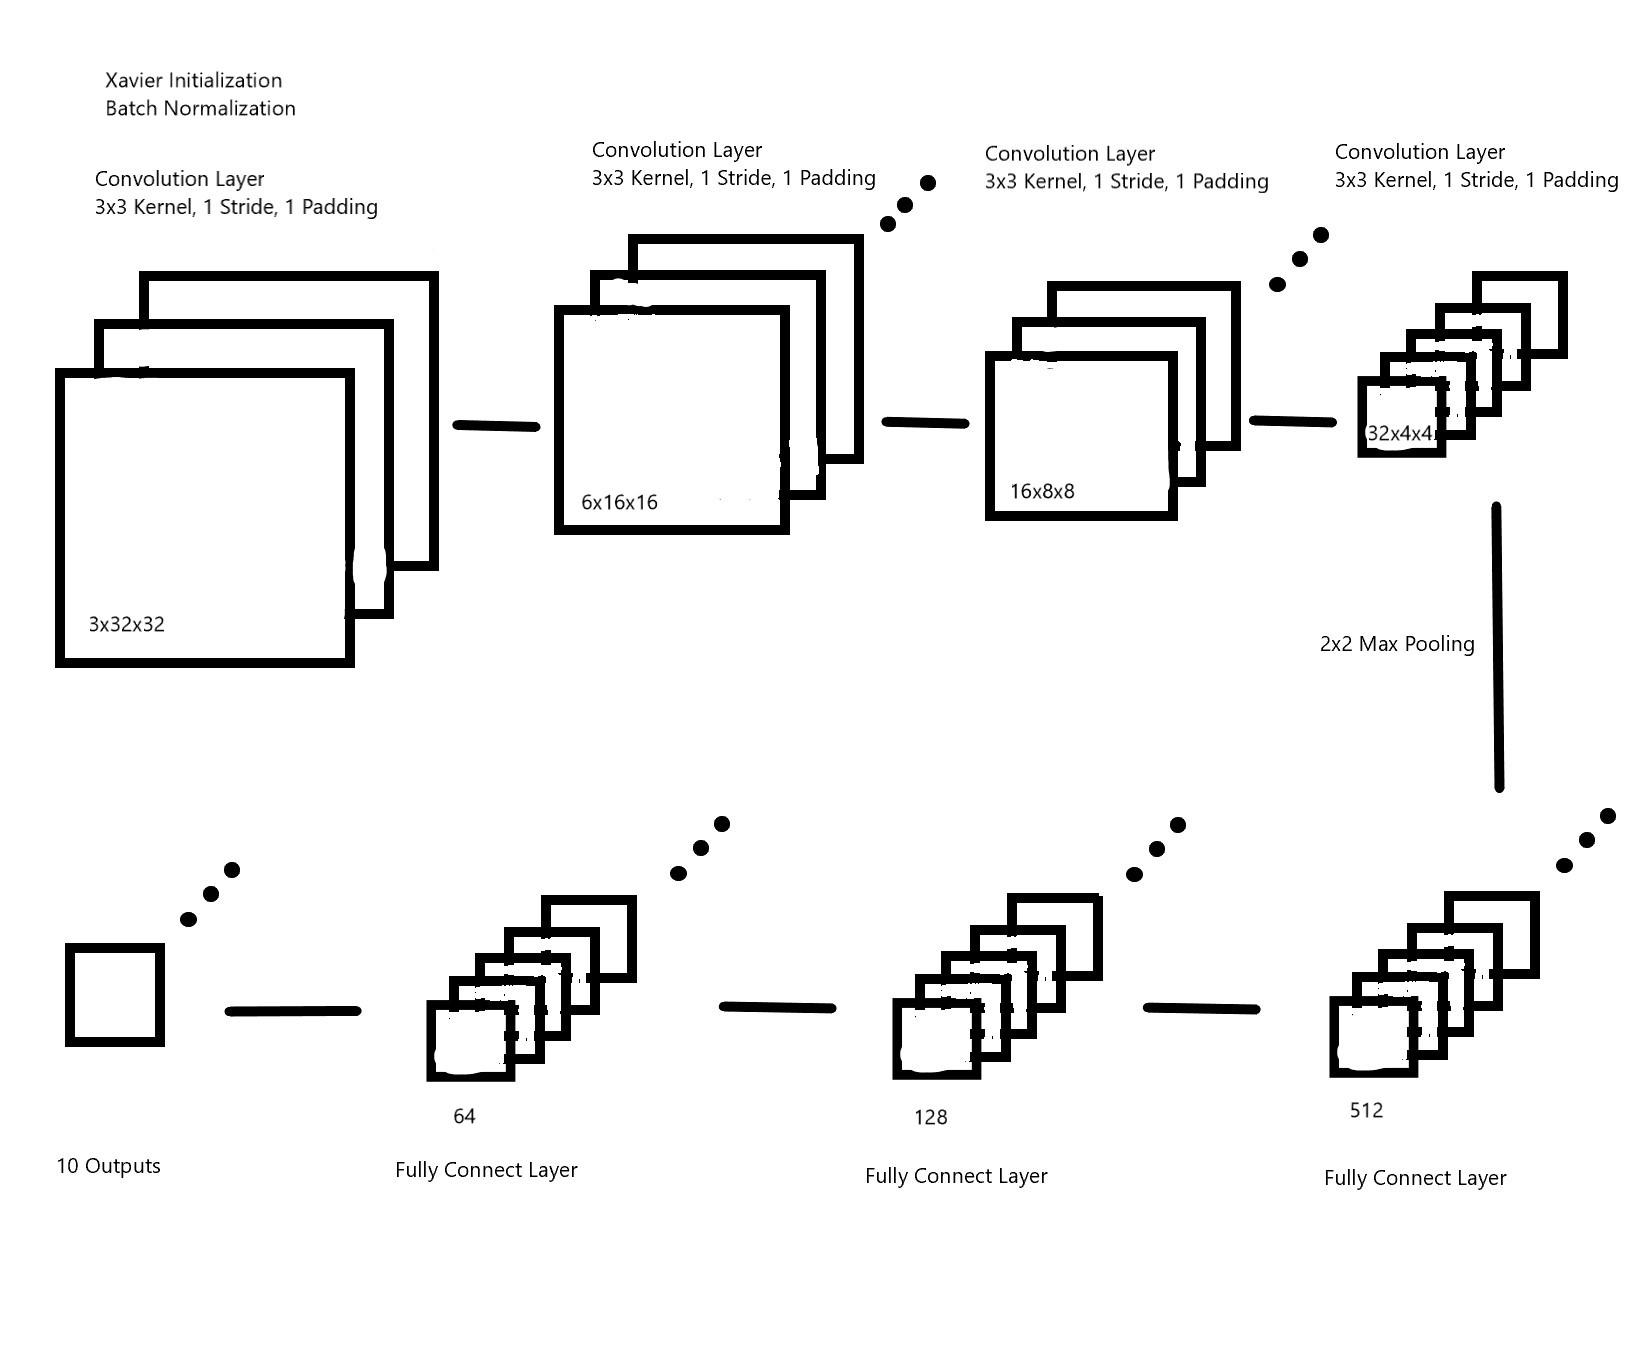
\includegraphics[width=6cm]{selfdiag.jpg} }}
    \caption{Self-built Model}
    \label{fig:self}
\end{figure}
 We also use Xavier initialization to keep the initial weights to be "just right". If the weights are 
 too small, the gradient will be too small. If the weights are too large, then the activation function 
 will be saturated causing the gradient to be small. \
 
 Finally, we use Adam Optimization instead of stochastic gradient descent. Adam Optimizer takes advantage
 of both Adaptive Gradient Algorithm and Root Mean Square Propagation. 
 Therefore, pooling operations have been essential for the success of current convolutional networks.


 \subsection{GoogLeNet Model }
We used part of GoogLeNet to train our model. GoogLeNet use Inception architecture in their models as shown in \figref{goog}. In inception model, they apply different filters on a single feature map and group them into one clusters of output. These clusters input of the next layer. According to \cite{Googlenet}, each unit from earlier layer describe some features of the input image and all passed to the next layer. Different feature maps are concatenated together into a single region and can be covered by a 1x1 convolution filter. Then several inception models are stacked on top of each other to form deep networks. Due memory efficience reason, they also proposed that it is beneficial to start using Inception modules at higher layers while keeping the lower layers in traditional convolutional fashion. In our work, we only took part of the whole GoogLeNet, first due to computation limitation and second the image size for Cifar is 32x32 compare to their 224x224 size. I also shrinked the size of convolution kernel at lower layer to take some more local features.
 \begin{figure}[h]
    \centering
    \subfloat[Accuracy vs. Epoch]{{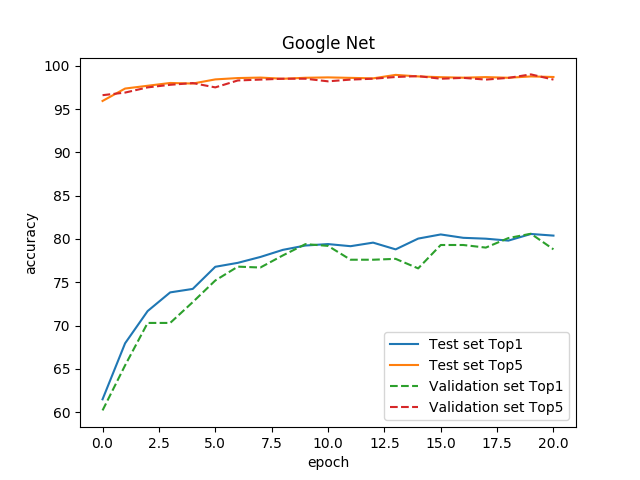
\includegraphics[width=6cm]{goolenet.png} }}
    \qquad
    \subfloat[GooLeNet Diagram]{{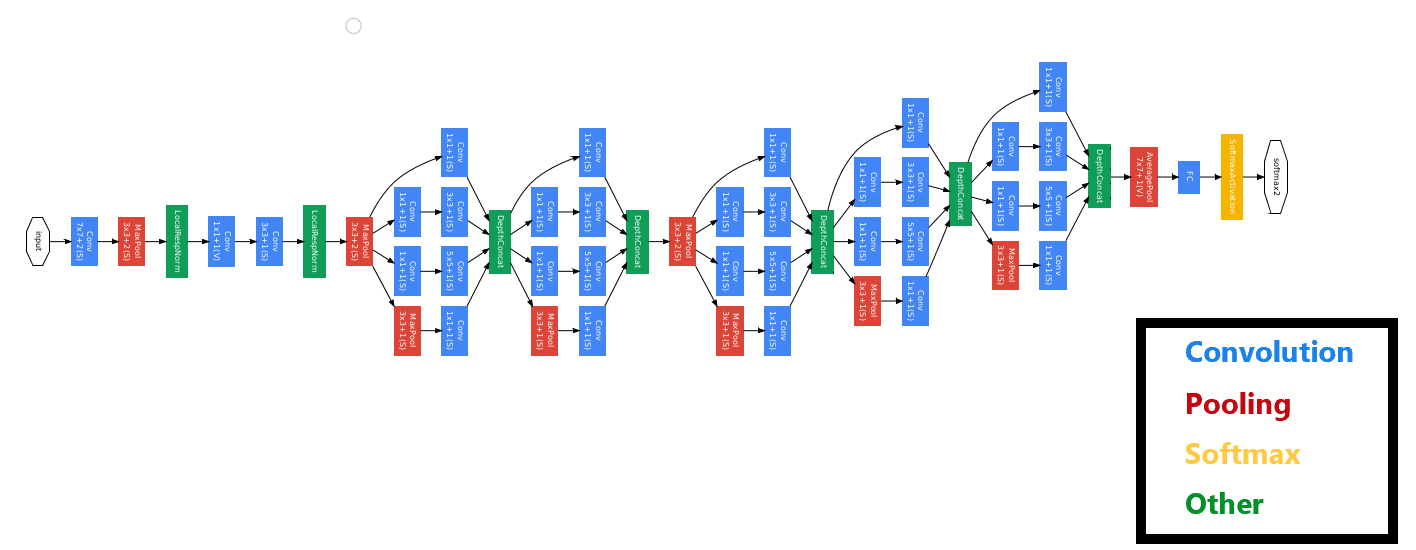
\includegraphics[width=6cm]{goodiag.png} }}
    \caption{GooLeNet Model}
    \label{fig:goog}
\end{figure}

\subsection{Discussion}
We first tried different parameters for self-build network. First, we tried to change kernel
size to 5,5,3 for three layers. The top5 accuracy drops from $97\%$ to $95\%$. As AlexNet originally 
suggested, we tried 11x11 kernel. However, the accuracy also drops. We suspects that in this dataset
local features are more preferred. \

Then, we replaced stochastic gradient descent with Adam. The accuracy raised from $94.1\%$ to $97.4\%$. It also takes less epochs to converge. As suggested in \cite{adam}, the step-size is approximately bounded by the step-size hyper-parameter and parameters update are invariant to re-scaling of gradient. Therefore, it can both speed up the learning process especially when it is about to converge and increase accuracy. \

We also tried Leak ReLU activation function and different sizes of maxpooling. However, the difference in accuracy and training speed is not noticeable. With leak ReLU, accuracy drop from $97\%$ to $96.2\%$ which is surprising since theoretically, leak ReLU should have better performance than regular ReLU.  

Generally, by comparing AlexNet, GoogLeNet and our self-built net, it is clear that GoogLeNet performs best, and AlexNet performs better than our self-built architecture. The difference between an AlexNet and our self-built architecture is that self-built net has three convolutional layer and three fully-connected layer, while AlexNet has five convolutional layer and three fully-connected layer. Their difference of two convolutional layers has result in different accuracies vs epochs, with AlexNet outperforms self-built net by 1.1\%. This simple comparison shows that given sufficient training data, a more complex function can be learned and enables the networks to more easily discriminate between different classes. The advantage of multiple layers is that they can learn features at various levels of abstraction, and are much better at generalization. This is also why in the space of 4 years, deep CNN develops from AlexNet to Residual nets (1000 layers).

From the accuracy plot for both AlexNet and GoogLeNet, we can see that GoogLeNet has a better performance compare to AlexNet. GoogLeNet is much deeper than AlexNet and takes advantage of Inception models which allows a significant amount of units in each layer. Increasing feature map can help the model to perform better and using inception model both local and global features can be captured through difference convolution kernel. Based on \cite{Googlenet}, the 1�1 convolutions are used to compute reductions before the expensive 3�3 and 5�5 convolutions. 
In terms of computation speed, the training time for GoogLeNet is doubled compare to AlexNet despite it is almost four times deeper than AlexNet. This leads to the another advantage of Inception architecture. GoogLeNet consists of several small parallel convolutions which can dramatically reduce the size of learnable parameter. Original GoogLeNet consisted of a 22 layer deep CNN but only as 4 million parameters, compare to AlexNet which has 60 million parameters. 
However, the model of GoogLeNet is not very intuitive compare to AlexNet. It is also harder to tune the parameters such as kernel size, stride, and convolution layer. It also takes GoogLeNet longer to converge.

% \section{Transfer Learning}
\IfFileExists{xxx_mainb}{\section{Transfer Learning}
Transfer learning is the method of applying a trained model on another dataset with similar traits. One popular application is to use it on image classification on small datasets that have insufficient number of labeled samples. Since deep convolutional networks trained on large-scale datasets learn universal features of images, it is a common practice to use the convolutional layers of the deep network as a feature extractor. Then by retraining the features on a simple single or multi layer network, one can train a image classifier on a small dataset.

\subsection{VGG16 Model}
For our task, we use the VGG16 model. VGG16 is a very deep convolutional network for large scale image recognition proposed in \cite{Simon}. It is a popular network, apart from AlexNet and GoogLeNet. The architecture of the network is shown in Figure \ref{vgg}.
\begin{figure}[H]
	\centering
	\includegraphics[width=8cm]{vgg16.png}%
	\caption{VGG16 Net Diagram \cite{vgg16fig}}
 	\label{vgg}
\end{figure}
The network consists of 16 layers of weights. The first 13 layers are convolutional layers stacked on top of each other. They extract the features of the images. The last 3 layers are linear layers, which is the classifier for the retrieved features.

\subsubsection{Dataset and Setup}
The dataset we are using is the Caltech-256 \cite{caltech}. It consists of 30607 images distributed over 257 classes. We ignore the "clutter" class and use the remaining 256 classes. From the dataset, we extract 40 images per class. 28 images are taken as our test set, the next 4 images are our validation set and the last 8 images are our test set.
 
To train a classifier on this smaller dataset, we substitute the last layer of the model to a 4096x256 linear layer. The previous layers are fixed and no weight updates are performed. 

We use cross-entropy loss function and Adam optimizer to train the new last layer of the model with mini-batch learning. Early stopping is performed with the tolerance of 10 iterations. We also anneal the learning rate with the following equation: 
\begin{equation}
\mu_t = \dfrac{\mu_0}{1+t/T}
\end{equation}

The parameters of our experiments are show in Table \ref{tab-trans1}. The model converges after 10 epochs, with the train accuracy of 90.04\%, validation accuracy of 72.27\% and test accuracy of 75.54\%

\begin{table}[H]
	\caption{Experiment Parameters}
	\centering
	\begin{tabular}{cc}
		\toprule
		%\multicolumn{5}{c}{Part}                   \\
		\cmidrule{1-2}
		Learning rate & 0.001\\
		\midrule
		Tolerance & 10\\
		\midrule
		T & 10\\
		\midrule
		Momentum & 0.9\\
		\midrule
		BatchSize & 32\\
		\bottomrule
	\end{tabular}
	\label{tab-trans1}
\end{table}

\subsubsection{Discussion}
The training results are shown in Figure \ref{fig-trans1}
%\begin{figure}[H]
%	\centering
%	\subfloat[Accuracy among epochs]{\includegraphics[width=6cm]{trans_correct.png}}%
%	\qquad
%	\subfloat[Loss among epochs]{\includegraphics[width=6cm]{trans_loss.png}}\\%
%	\caption{Accuracy and loss over epochs}
%	\label{fig-trans1}
%\end{figure}

\begin{figure}[H]
\centering
\subcaptionbox{Accuracy among epochs}{\includegraphics[width=0.5\textwidth]{trans_correct.png}}%
\subcaptionbox{Loss among epochs}{\includegraphics[width=0.5\textwidth]{trans_loss.png}}\\%
\caption{Accuracy and loss over epochs}
\label{fig-trans1}
\end{figure}



The overall performance of the new model is decent, considering we are only giving the model 28 images per class, with a total amount of 256 classes. 

The train, validation and test accuracy and loss figures are also reasonable. All of them are monotonic and converge to a maximum/minimum value. 

That being said, there are two abnormalities that can be observed in the figure. One is the unusually high train accuracy. We can see that the training accuracy is much higher than the validation and test accuracy. The validation and training loss quickly converges at the 5th epoch, while the training loss is still decreasing. With a small dataset, limited samples per class are shown to the model, thus it is harder to generalize. We can deduce that the model is overfitting on the limited training samples.

Another is the exceptionally higher validation and test accuracy in the first two epochs. Training accuracy is mostly only used to observe if the model is learning the training set and whether it is overfitting. To speed up computation, we estimate the train accuracy after each epoch by taking the average training accuracy over the mini-batches. Thus we do not need an extra forward pass after each epoch, but compute the training accuracy during the back-propagation process. The validation and test accuracy are calculated after each epoch. Thus the train accuracy is not collected from the same model as the validation and test accuracy. But as the model converges, the train accuracy also converges and is a good representation of the training performance. Because the model is learning at a very fast pace, for the first two epochs, the train accuracy is lower than the validation and test accuracy.

\section{Transfer Learning}
\subsection{Visualization}
Normally for convolutional neural network, visualization can be processed by some naive methods.
\begin{itemize}
\item Visualize the feature maps after convolutional block
\item Visualize the filters in the first convolutional block
\end{itemize}

Feature maps describe how neural network understand an image at certain level, and filters represent patterns the neural network tends to find in each layer. There are also other approaches using deconvolutional network and feature evolution mentioned in \cite{zeiler} to get deeper insights, but requiring for large computation cost. Here for simplicity, we just use the naive techniques described before.

\subsubsection{Experiment Setup}
We still used the pruned VGG16 network mentioned in Section 3.1.1. The parameters of the model are all pre-trained. The weights and bias in conv blocks and the first linear layer are copied from the parameters set trained from ImageNet, and the parameters in the last $4096\times 256$ linea layer is acquired from the Caltech-256 dataset, through transfer learning process.

The visualization of the feature maps is depend on input images, as this represents the activation result after the neural network model receiving the input. In practice, we use an image as input, and let neural network do the feedforward process to acquire the activation result. The activation result of a convolutional layer is a tensor with size $K \times W\times H$, where $K$ is the number of filters, and $W$ and $H$ are size of the feature maps. At last, we pick up a subset of feature maps from the first and last convolutional layers, then plot them as heatmaps.

The weights in filters at first layer can be seen as a $3\times K \times W \times H$ tensor, which indicates the input images have 3 channels(RGB), $K$ filters in first layer and will generate feature maps with width of $W$ and height of $H$. For each filter, we can visualize it as a RGB image, which specifies its preference among different color channels. Although we can also visualize filters in layers afterwards, their inputs are not in pixel-place, hence rarely can provide any intuition to us. Therefore we omit this procedure, and only focus on filters in the first convolutional layer.

\subsubsection{Discussion}
First we picked up a specific image (billiards) as input, shown in Figure \ref{fig-input}

\begin{figure}[H]
  \centering
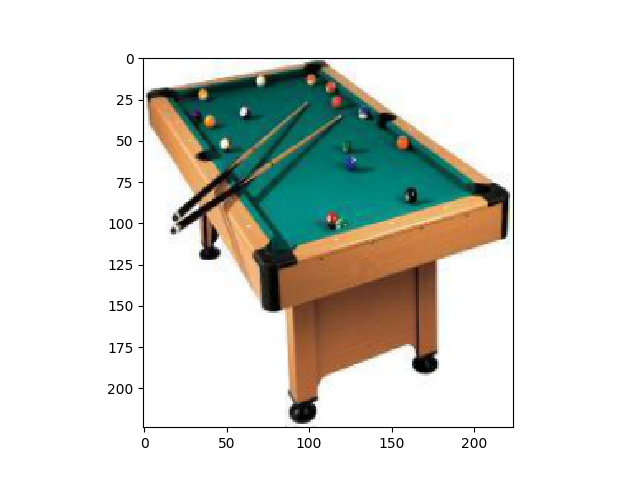
\includegraphics[width=0.5\textwidth]{raw_input.png}
  \caption{The input image}
  \label{fig-input}
\end{figure}

Follows are some results for visualization of activations, represented in headmaps. The activation for the first convolutional layer has size $224\times 224$, whereas the activation for the last convolutional layer has size $14\times 14$. The lighter yellow color indicated strong activation in that area, and the darker blue color means low interest in those regions.

%TODO activation show

\begin{figure}[H]
\centering
\subcaptionbox{from filter 6 (blue vertical line )}{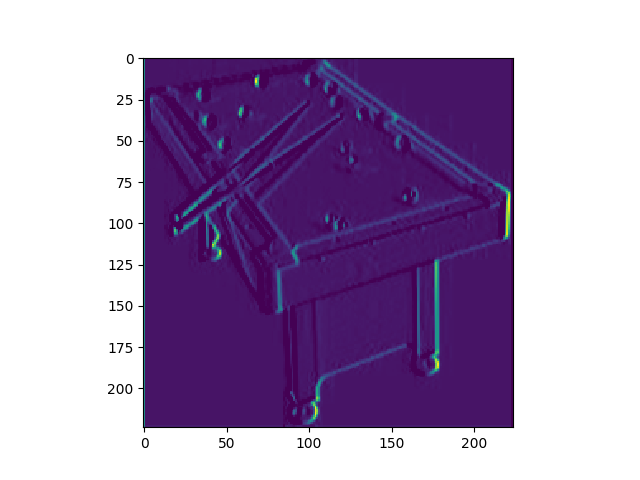
\includegraphics[width=0.5\textwidth]{first_conv6.png}}%
\subcaptionbox{from filter 27 (dark corner)}{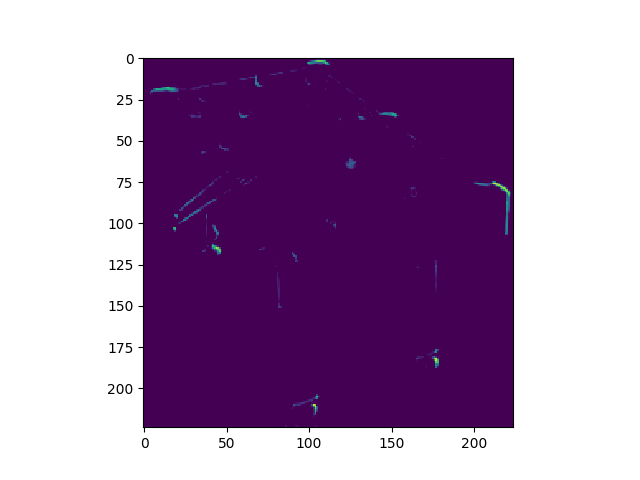
\includegraphics[width=0.5\textwidth]{first_conv27.png}}\\%
\subcaptionbox{from filter 15 (green surface)}{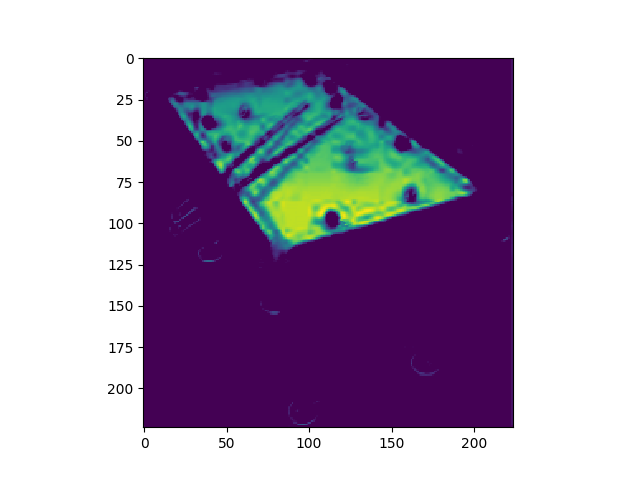
\includegraphics[width=0.5\textwidth]{first_conv15.png}}%
\subcaptionbox{from filter 47 (yellow surface)}{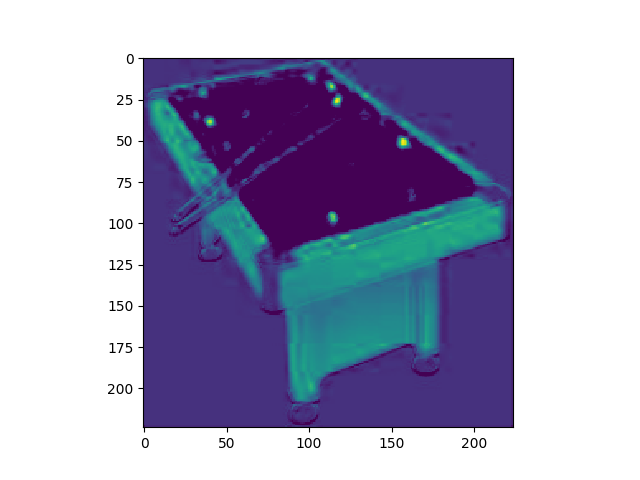
\includegraphics[width=0.5\textwidth]{first_conv47.png}}%
\caption{Activations from different filters in first conv layer}
\label{fig-acti-in}
\end{figure}

We can see that the activations from the first convolutional layer is very illustrated in Figure \ref{fig-acti-in}. The majority of them are just basic geometry feautures extracted by some line detectors(filter 6), corner detectors(filter 27) or texture detectors with repect to differnt colors (compare filter 15 and filter 47). These visualized activation maps are with sharp distinction. While the activations from the last convolutional layer have smaller size and hence are hard to read, shown in Figure \ref{fig-acti-out}. Their inputs are not in pixel-space so we can just infer they are judging some higher-level features from certain interested regions (the contour and content are all blurred, comparing to the first layer activation)

\begin{figure}[H]
\centering
\subcaptionbox{from filter 34 }{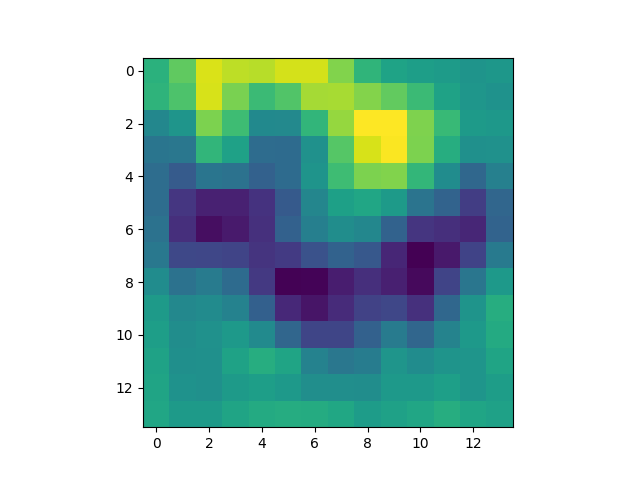
\includegraphics[width=0.25\textwidth]{last_conv34.png}}%
\subcaptionbox{from filter 70}{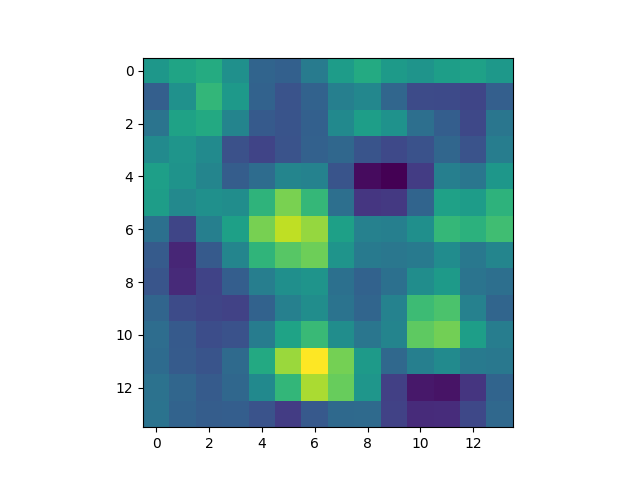
\includegraphics[width=0.25\textwidth]{last_conv70.png}}%
\subcaptionbox{from filter 135}{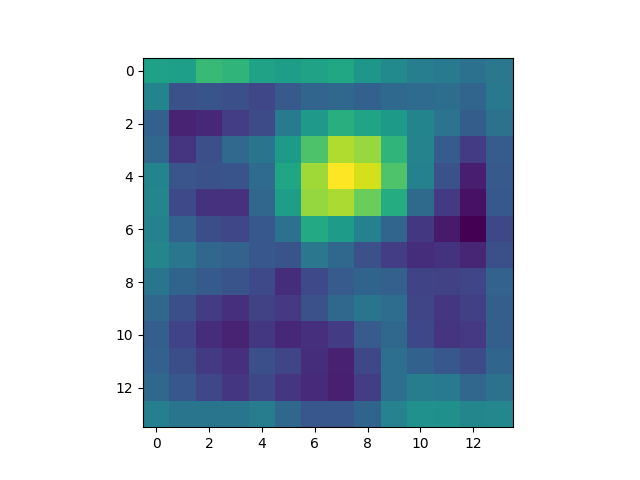
\includegraphics[width=0.25\textwidth]{last_conv135.png}}%
\subcaptionbox{from filter 282}{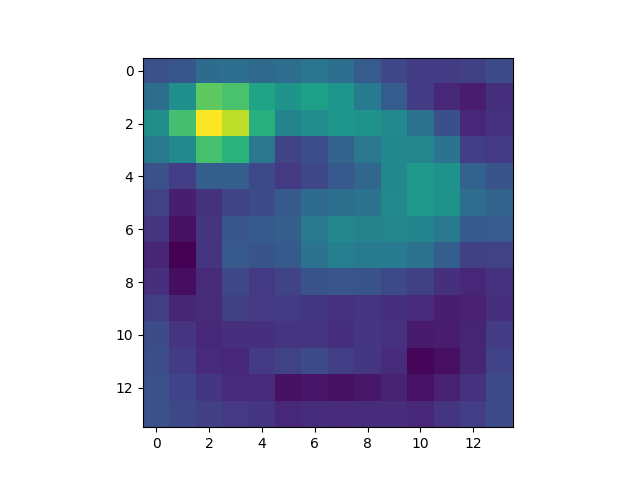
\includegraphics[width=0.25\textwidth]{last_conv282.png}}%
\caption{Activations from different filters in the last conv layer}
\label{fig-acti-out}
\end{figure}


%TODO weights show
%diversity in color and gradient
Then we take a look at the weights of the filters. In Figure\ref{fig-filter-in1} can we see that the diversity of filters in color and gradient of pixel intensity(patterns). It is this diversity to make sure the first layer can extract as much features as possible and propagate them to the next convolutional block. Also, to clearify their specific meanings, we combined the filter with their corresponding activation map to better understand their functions in the first convolutional layer, display them in Figure \ref{fig-filter-in}. Filters are visualized in size $3\times 3$ with RGB channels to denote their color preference. As we can see, filter 6 is recognizing vertical lines in the image, most favor in dark blue (since we shift all the weights to non-negative, the lighter color in yellow just means it doesn't like yellow, and darker blue means it heavily chases on that color), filter 27 is for corner of upper right angle in red and blue, filter 15 is for green surface and filter 47 for red and yellow.


\begin{figure}[H]
\centering
\subcaptionbox{filter 00}{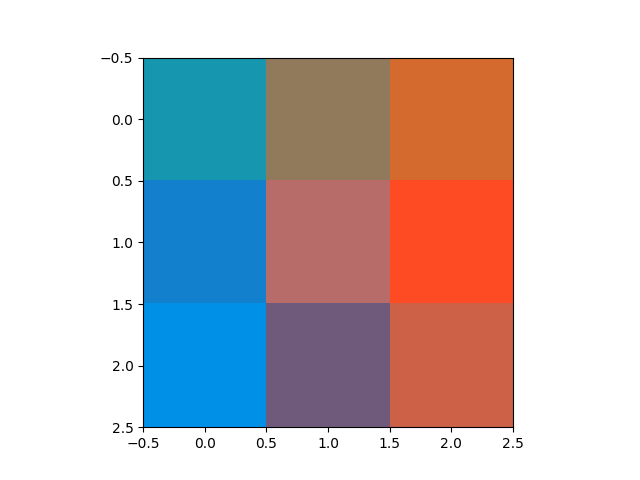
\includegraphics[width=0.125\textwidth]{filter0.png}}%
\subcaptionbox{filter 01}{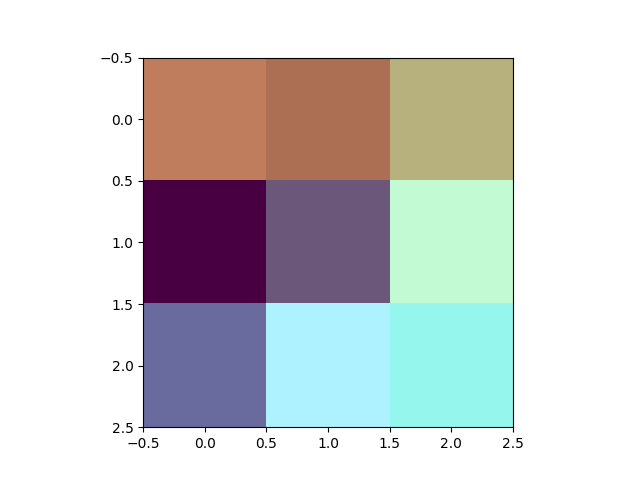
\includegraphics[width=0.125\textwidth]{filter1.png}}%
\subcaptionbox{filter 02}{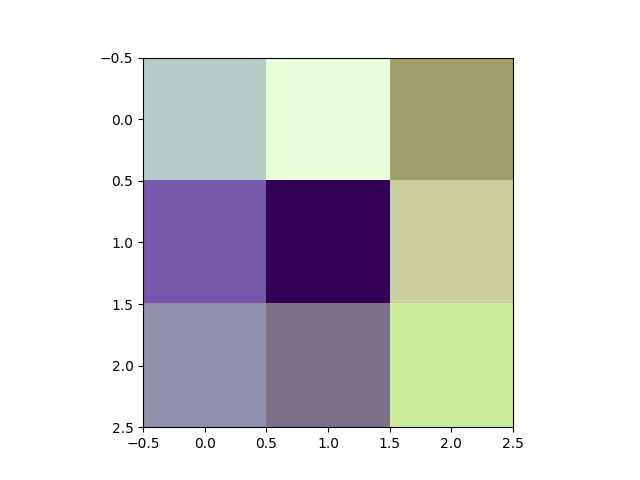
\includegraphics[width=0.125\textwidth]{filter2.png}}%
\subcaptionbox{filter 03}{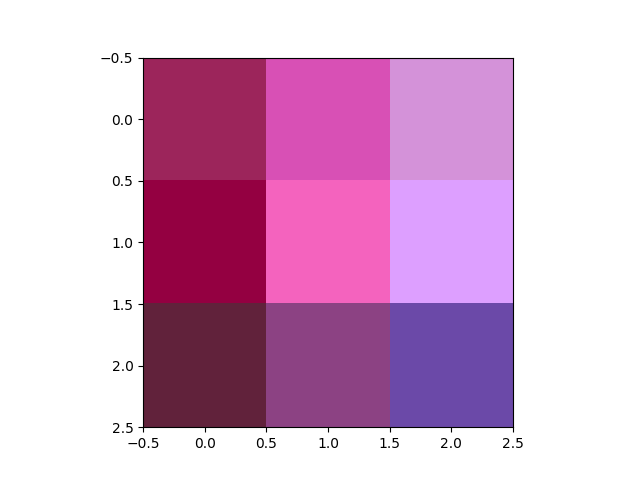
\includegraphics[width=0.125\textwidth]{filter3.png}}%
\subcaptionbox{filter 04}{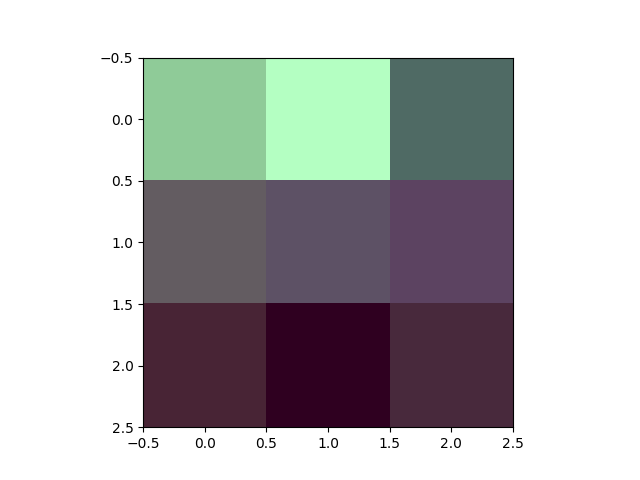
\includegraphics[width=0.125\textwidth]{filter4.png}}%
\subcaptionbox{filter 05}{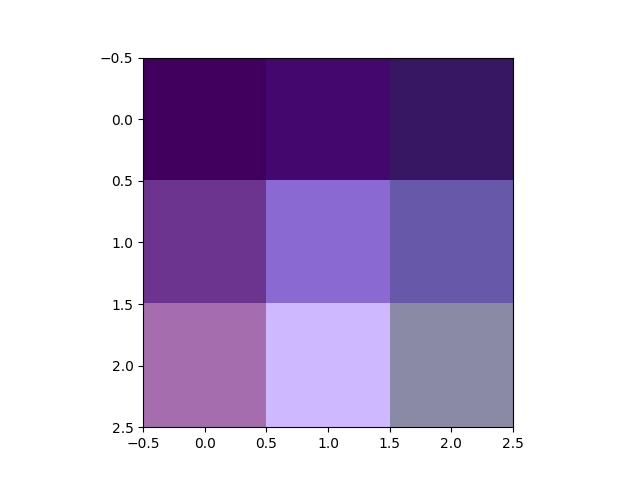
\includegraphics[width=0.125\textwidth]{filter5.png}}%
\subcaptionbox{filter 06}{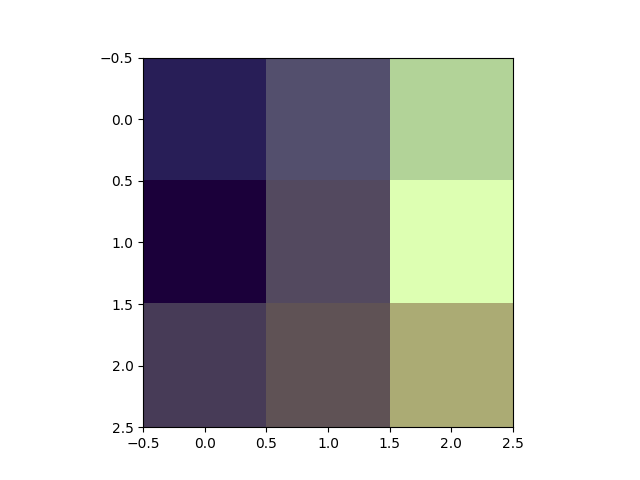
\includegraphics[width=0.125\textwidth]{filter6.png}}%
\subcaptionbox{filter 07}{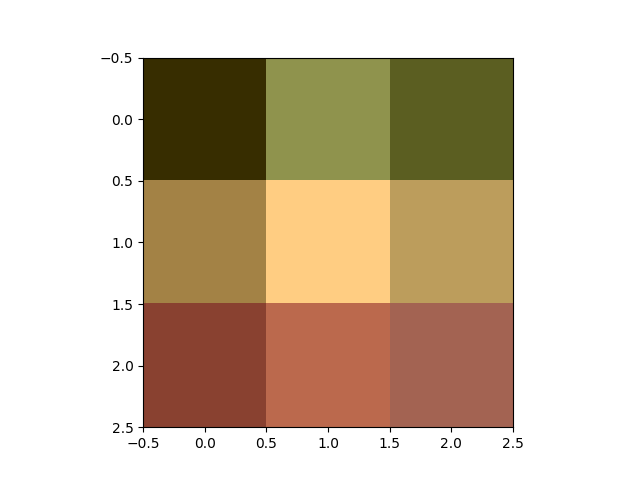
\includegraphics[width=0.125\textwidth]{filter7.png}}\\%

\subcaptionbox{filter 8}{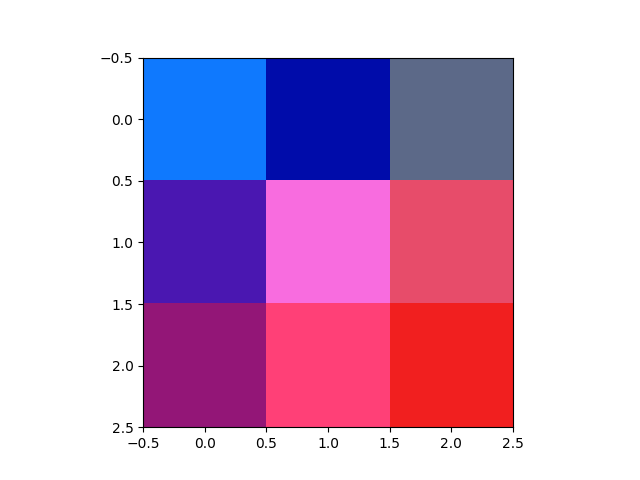
\includegraphics[width=0.125\textwidth]{filter8.png}}%
\subcaptionbox{filter 9}{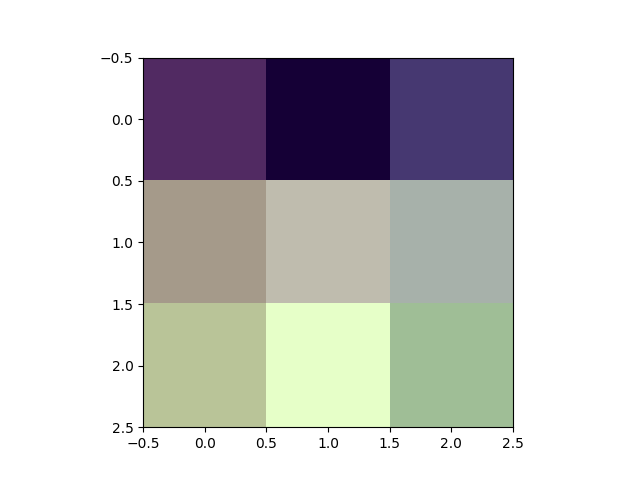
\includegraphics[width=0.125\textwidth]{filter9.png}}%
\subcaptionbox{filter 10}{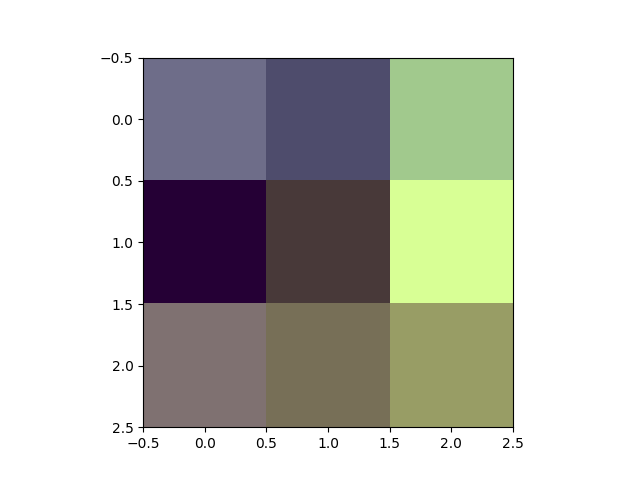
\includegraphics[width=0.125\textwidth]{filter10.png}}%
\subcaptionbox{filter 11}{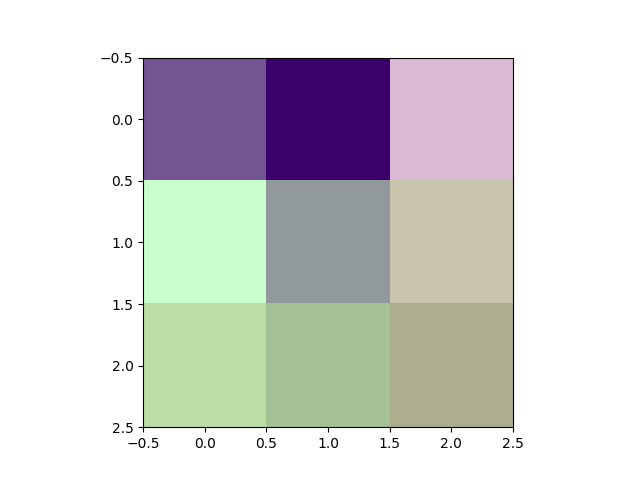
\includegraphics[width=0.125\textwidth]{filter11.png}}%
\subcaptionbox{filter 12}{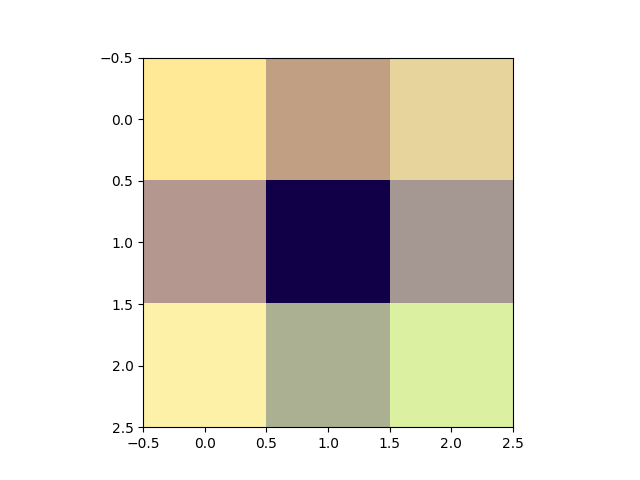
\includegraphics[width=0.125\textwidth]{filter12.png}}%
\subcaptionbox{filter 13}{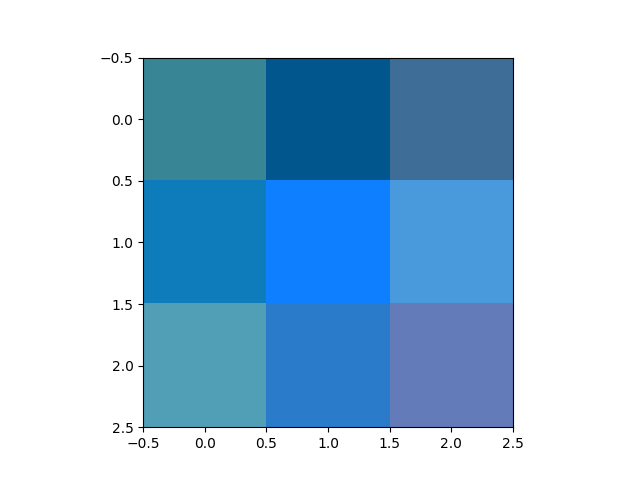
\includegraphics[width=0.125\textwidth]{filter13.png}}%
\subcaptionbox{filter 14}{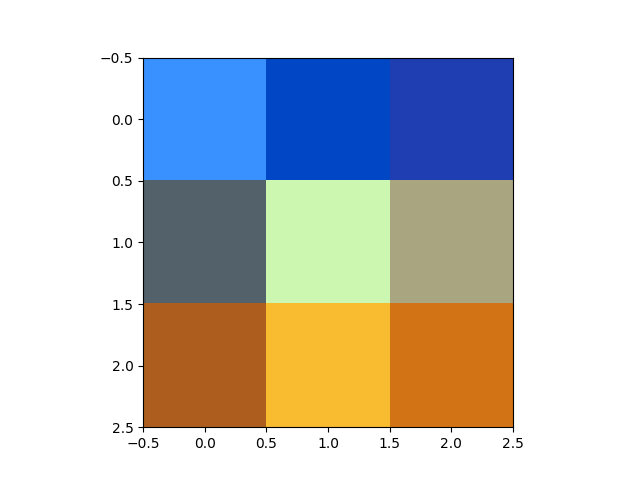
\includegraphics[width=0.125\textwidth]{filter14.png}}%
\subcaptionbox{filter 15}{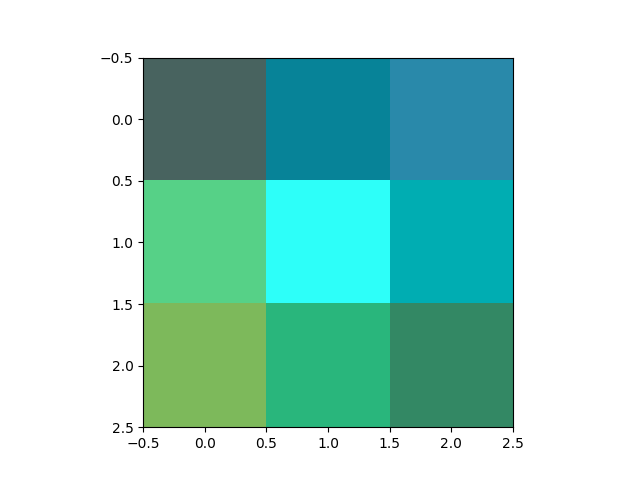
\includegraphics[width=0.125\textwidth]{filter15.png}}\\%

\subcaptionbox{filter 16}{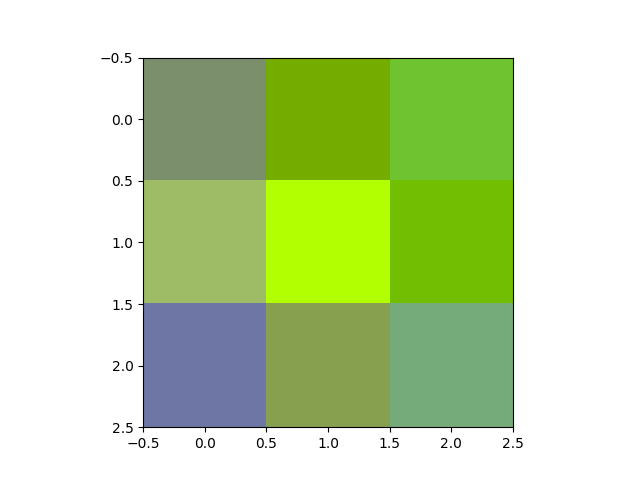
\includegraphics[width=0.125\textwidth]{filter16.png}}%
\subcaptionbox{filter 17}{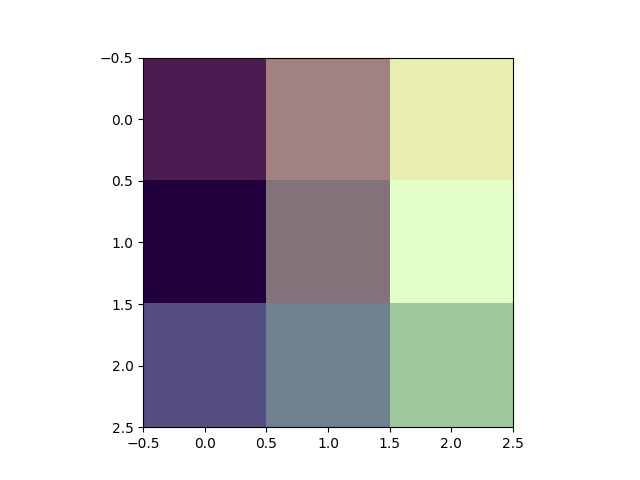
\includegraphics[width=0.125\textwidth]{filter17.png}}%
\subcaptionbox{filter 18}{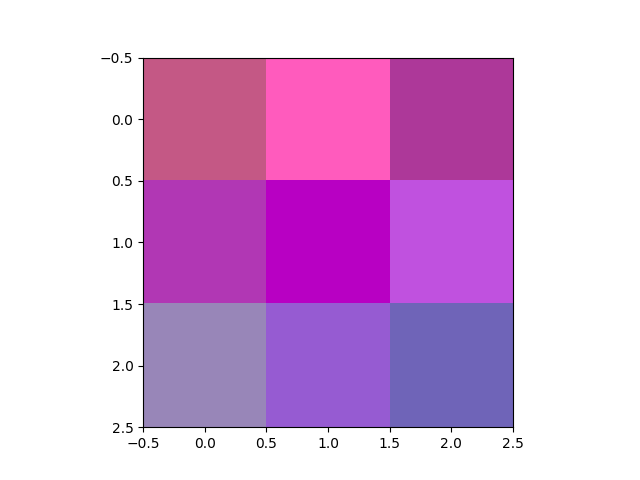
\includegraphics[width=0.125\textwidth]{filter18.png}}%
\subcaptionbox{filter 19}{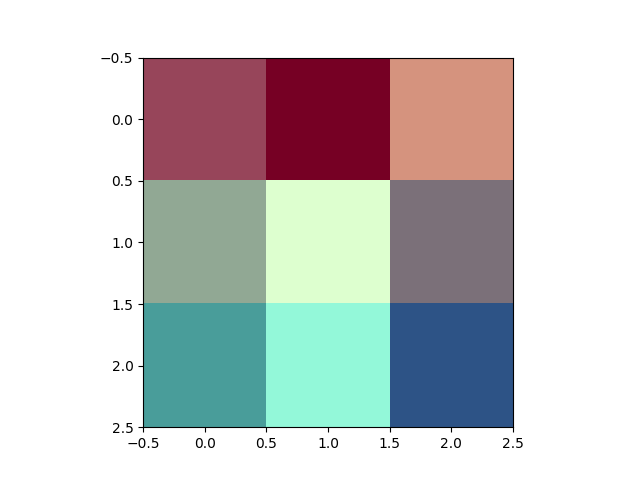
\includegraphics[width=0.125\textwidth]{filter19.png}}%
\subcaptionbox{filter 20}{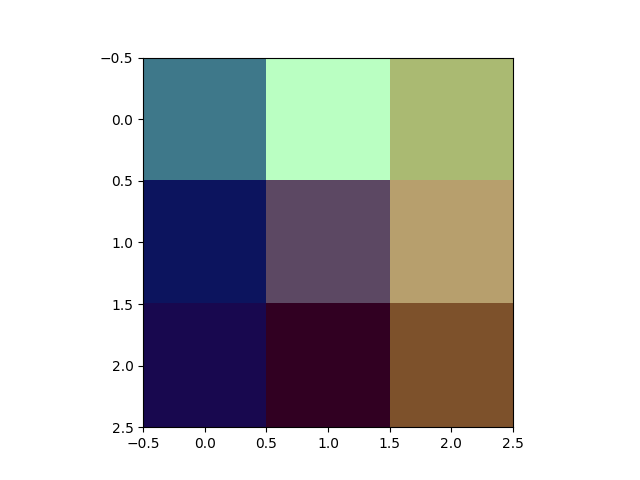
\includegraphics[width=0.125\textwidth]{filter20.png}}%
\subcaptionbox{filter 21}{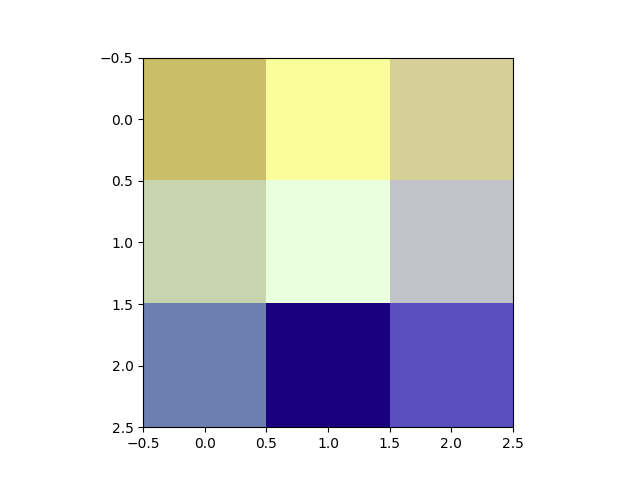
\includegraphics[width=0.125\textwidth]{filter21.png}}%
\subcaptionbox{filter 22}{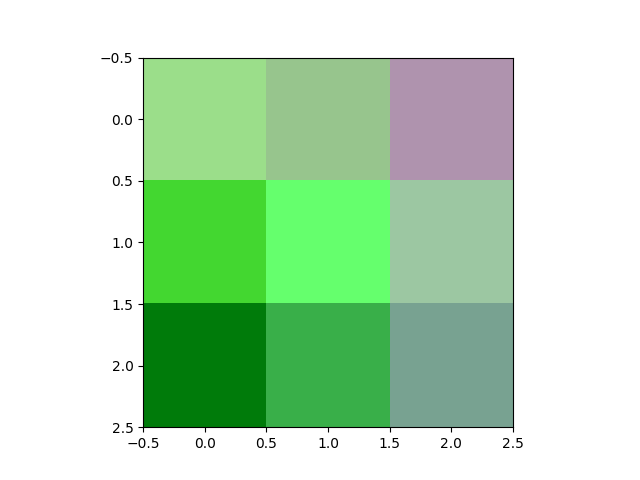
\includegraphics[width=0.125\textwidth]{filter22.png}}%
\subcaptionbox{filter 23}{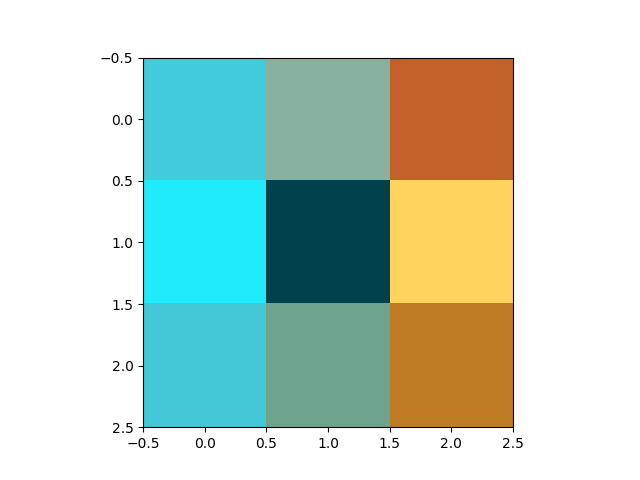
\includegraphics[width=0.125\textwidth]{filter23.png}}\\%

\subcaptionbox{filter 24}{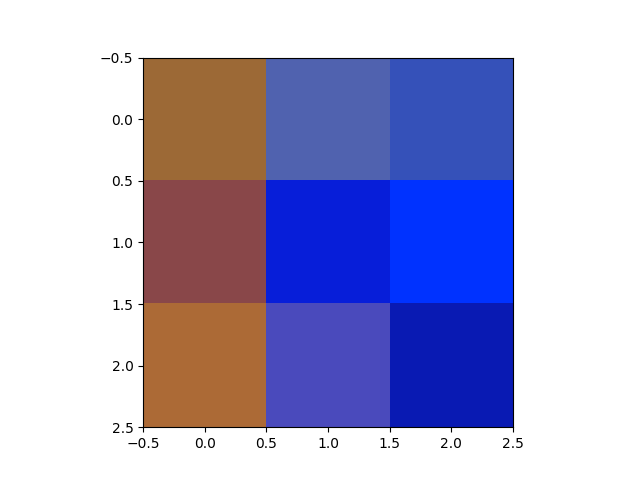
\includegraphics[width=0.125\textwidth]{filter24.png}}%
\subcaptionbox{filter 25}{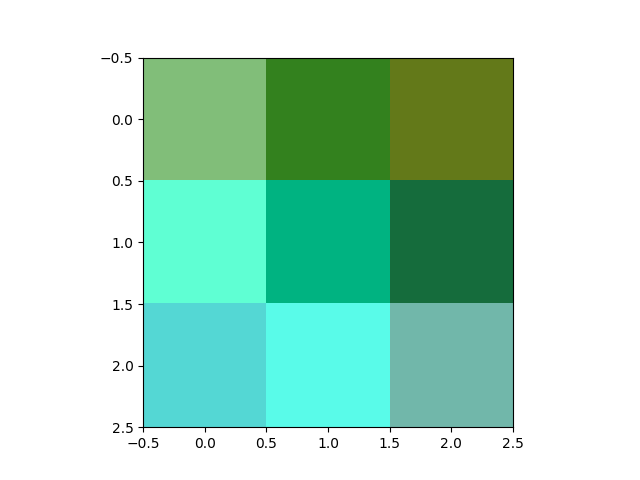
\includegraphics[width=0.125\textwidth]{filter25.png}}%
\subcaptionbox{filter 26}{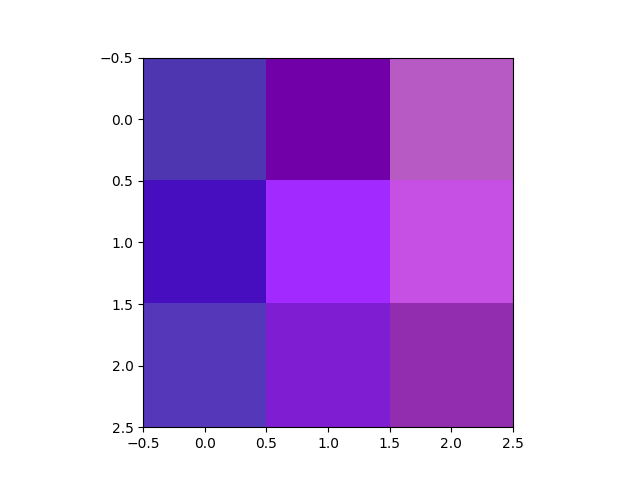
\includegraphics[width=0.125\textwidth]{filter26.png}}%
\subcaptionbox{filter 27}{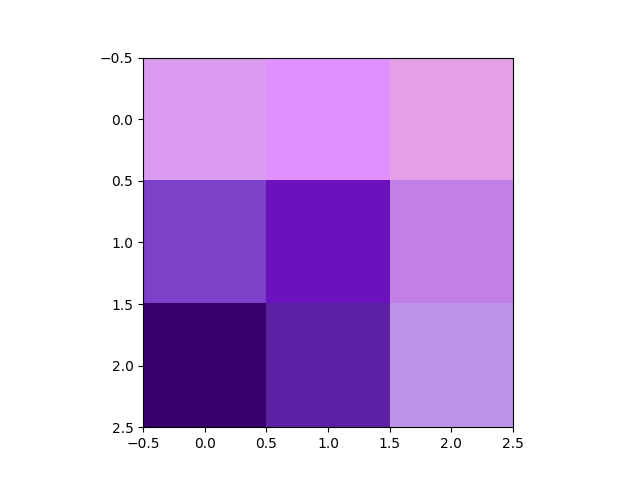
\includegraphics[width=0.125\textwidth]{filter27.png}}%
\subcaptionbox{filter 28}{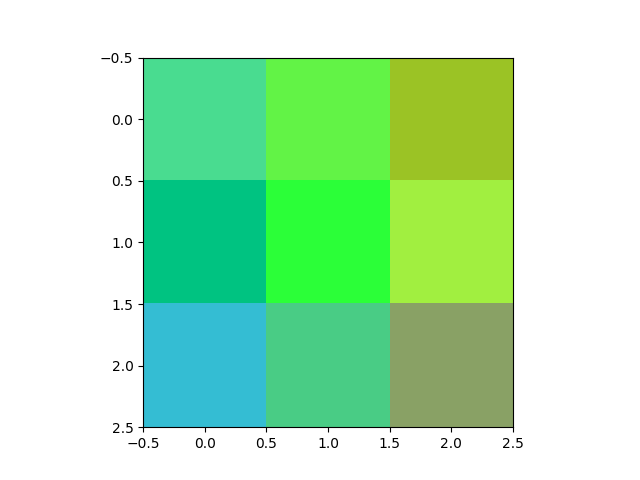
\includegraphics[width=0.125\textwidth]{filter28.png}}%
\subcaptionbox{filter 29}{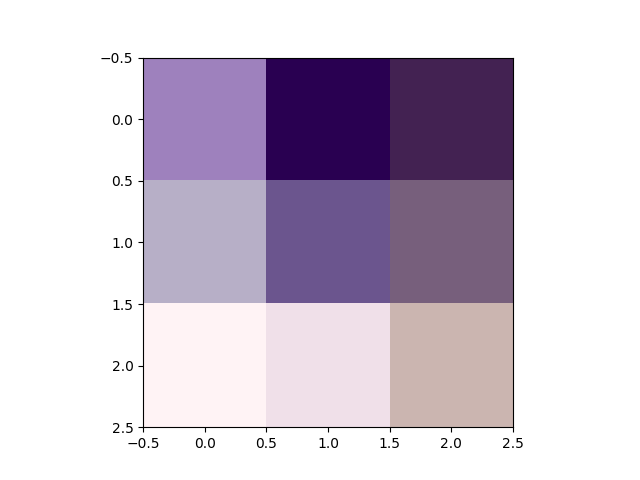
\includegraphics[width=0.125\textwidth]{filter29.png}}%
\subcaptionbox{filter 30}{\includegraphics[width=0.125\textwidth]{filter30.png}}%
\subcaptionbox{filter 31}{\includegraphics[width=0.125\textwidth]{filter31.png}}\\%

\subcaptionbox{filter 32}{\includegraphics[width=0.125\textwidth]{filter32.png}}%
\subcaptionbox{filter 33}{\includegraphics[width=0.125\textwidth]{filter33.png}}%
\subcaptionbox{filter 34}{\includegraphics[width=0.125\textwidth]{filter34.png}}%
\subcaptionbox{filter 35}{\includegraphics[width=0.125\textwidth]{filter35.png}}%
\subcaptionbox{filter 36}{\includegraphics[width=0.125\textwidth]{filter36.png}}%
\subcaptionbox{filter 37}{\includegraphics[width=0.125\textwidth]{filter37.png}}%
\subcaptionbox{filter 38}{\includegraphics[width=0.125\textwidth]{filter38.png}}%
\subcaptionbox{filter 39}{\includegraphics[width=0.125\textwidth]{filter39.png}}\\%

\subcaptionbox{filter 40}{\includegraphics[width=0.125\textwidth]{filter40.png}}%
\subcaptionbox{filter 41}{\includegraphics[width=0.125\textwidth]{filter41.png}}%
\subcaptionbox{filter 42}{\includegraphics[width=0.125\textwidth]{filter42.png}}%
\subcaptionbox{filter 43}{\includegraphics[width=0.125\textwidth]{filter43.png}}%
\subcaptionbox{filter 44}{\includegraphics[width=0.125\textwidth]{filter44.png}}%
\subcaptionbox{filter 45}{\includegraphics[width=0.125\textwidth]{filter45.png}}%
\subcaptionbox{filter 46}{\includegraphics[width=0.125\textwidth]{filter46.png}}%
\subcaptionbox{filter 47}{\includegraphics[width=0.125\textwidth]{filter47.png}}\\%

\subcaptionbox{filter 48}{\includegraphics[width=0.125\textwidth]{filter48.png}}%
\subcaptionbox{filter 49}{\includegraphics[width=0.125\textwidth]{filter49.png}}%
\subcaptionbox{filter 50}{\includegraphics[width=0.125\textwidth]{filter50.png}}%
\subcaptionbox{filter 51}{\includegraphics[width=0.125\textwidth]{filter51.png}}%
\subcaptionbox{filter 52}{\includegraphics[width=0.125\textwidth]{filter52.png}}%
\subcaptionbox{filter 53}{\includegraphics[width=0.125\textwidth]{filter53.png}}%
\subcaptionbox{filter 54}{\includegraphics[width=0.125\textwidth]{filter54.png}}%
\subcaptionbox{filter 55}{\includegraphics[width=0.125\textwidth]{filter55.png}}\\%

\subcaptionbox{filter 56}{\includegraphics[width=0.125\textwidth]{filter56.png}}%
\subcaptionbox{filter 57}{\includegraphics[width=0.125\textwidth]{filter57.png}}%
\subcaptionbox{filter 58}{\includegraphics[width=0.125\textwidth]{filter58.png}}%
\subcaptionbox{filter 59}{\includegraphics[width=0.125\textwidth]{filter59.png}}%
\subcaptionbox{filter 60}{\includegraphics[width=0.125\textwidth]{filter60.png}}%
\subcaptionbox{filter 61}{\includegraphics[width=0.125\textwidth]{filter61.png}}%
\subcaptionbox{filter 62}{\includegraphics[width=0.125\textwidth]{filter62.png}}%
\subcaptionbox{filter 63}{\includegraphics[width=0.125\textwidth]{filter63.png}}\\%
\caption{Filters in first conv layer}
\label{fig-filter-in1}
\end{figure}

\begin{figure}[H]
\centering
\subcaptionbox{filter 6 (blue line)}{\includegraphics[width=0.25\textwidth]{filter6.png}}%
\subcaptionbox{activation from filter 6}{\includegraphics[width=0.25\textwidth]{first_conv6.png}}%
\subcaptionbox{filter 27 (dark corner)}{\includegraphics[width=0.25\textwidth]{filter27.png}}%
\subcaptionbox{activation from filter 27}{\includegraphics[width=0.25\textwidth]{first_conv27.png}}\\%

\subcaptionbox{filter 15 (green surface)}{\includegraphics[width=0.25\textwidth]{filter15.png}}%
\subcaptionbox{activation from filter 15 }{\includegraphics[width=0.25\textwidth]{first_conv15.png}}%
\subcaptionbox{filter 47 (yellow surface)}{\includegraphics[width=0.25\textwidth]{filter47.png}}%
\subcaptionbox{activation from filter 47 }{\includegraphics[width=0.25\textwidth]{first_conv47.png}}%
\caption{Activations and corresponding filters in first conv layer}
\label{fig-filter-in}
\end{figure}

In general, activations from the filters indicate different convolutional layers in cascade  structured neural network model perform different tasks during the image classification process. The initial convolutional layers mainly focus on basic geometry features in image, like corners or lines. And the higher level convolutional layers tend to learn some semantic elements and components to help with image classification. The pixel level information is first transformed to lower level feature, then propagate to convolutional layers afterwards to higher level comprehension. And the diversity of filters in the first convolutional layers, both in color distribution and gradient of pixel intensity, guarantees that the information from the image can be maximum preserved and utilize to help downstream convolutional layers do the classfication.

\subsection{Feature Extraction}
In this section we are going to design experiement to illustrate how the depth of the convolutional neural network decides the classification performance. 

\subsubsection{Experiment Setup}
Here we reserved the former structure of the transfered-VGG16 net, and altered the two-layer fully connection layer to a single hidden layer with 1000 hidden units. The final layer is still kept as a softmax layer with 256 dimension output. The original VGG16 net has 5 convolutional blocks. We used the first 3, 4 and all 5 convolutional blocks respectively and calculated the classfication metrics. To get best accuracy in each cases, our learning rate is set as 0.0005 for 4 and 5 conv blocks, and 0.0001 for 3 conv blocks. Our annealing factor $T$ is set as 50. All other parameters are the same mentioned in Table \ref{tab-trans1}. We use the result from transfer learning part as our baseline.

\subsubsection{Discussion}
Different performances by using different numbers of conv blocks are shown in Table \ref{tab-cmp}. Here "i-conv" means using i conv blocks for classification, and "conv-i" means the i-th conv block in VGG16. We can see that using only part of (conv blocks of) pre-trained VGG model also can do the classification job, but in a very low accuracy. As the conv blocks numbers increasing, the accuracy increases sharply, from 29.74\% to 71.29\%. While adding another hidden layer or increasing the hidden units numbers don't improve the performance too much, just by several percentages. Also we can see that during training phase, the accuracy on training set of shallower model tends to reach closer to 1. This is because although the number of layers is less, the scale of output features from the last conv block is much bigger ($28\times 28\times 256=200704$ in 3-conv case) than the ($7\times 7\times 512=25088$ in 5-conv case) which result in more number of weighs in fully connected layer. And because we only have limited number of data on Caltech-256(30607 images), we can easily get overfit.

\begin{table}[H]
	\caption{Accuracy Comparison}
	\centering
	\begin{tabular}{|c|c|c|c|c|}
		\hline
		 & 3-conv & 4-conv & 5-conv & baseline\\
		\hline
		level-1 & conv-1   & conv-1   & conv-1   & conv-1\\
		\hline
		level-2 & conv-2   & conv-2   & conv-2   & conv-2\\
		\hline
		level-3 & conv-3   & conv-3   & conv-3   & conv-3\\
		\hline
		level-4 & fc(1000) & conv-4   & conv-4   & conv-4\\
		\hline
		level-5 & softmax  & fc(1000) & conv-5   & conv-5\\
        \hline
		level-6 &          & softmax  & fc(1000) & fc(4096)\\		
		\hline
		level-7 &          &          & softmax  & fc(4096)\\
		\hline
		level-8 &          &          &          & softmax\\
		\hline
		Train acc. &1.0000 & 1.0000   & 0.9993   & 0.9500 \\
		\hline
		Valid acc. &0.2822 & 0.5166   & 0.7129   & 0.7100 \\
		\hline		
		Test acc.  &0.2876 & 0.5322   & 0.7129   & 0.7554 \\
		\hline		
	\end{tabular}
	\label{tab-cmp}
\end{table}}{.}

\section{Conclusion}
In summary, out of the three models we implemented and after several experiments, we can conclude that GoogLeNet has the best performance. GoogLeNet is much deeper than the other two architectures and the training time is also longer, but it takes less epochs to converge. When comparing within the same architecture, say our self-built net, changing the kernel size from 3,3,3 to 5,5,3 results in accuracy drop. In AlexNet when changing kernel size from 5,5,3,3,3 to 11x11 also leads to accuracy drop. Adam optimizer proves to help increase the accuracy and speed up learning of the neural network, while Xavier initialization does not show obvious difference on results. Using different activation function and different sizes of maxpooling do not have a significant effect on accuracy results. 

\IfFileExists{xxx_concl}{%TODO

%Generally speaking, applying different tricks to neural networks does not affect much on the training results, say accuracy and loss. However, what needs to be taken into consideration is the trick parameter choices and acceleration effect tricks can have on training process. For example, weight initialization needs to be chosen randomly so that sigmoid is primarily activated in linear region.   
% 
%Moreover, the number of hidden nodes can have different effects on the training results. If the number of hidden nodes are too large or too small, the accuracy will drop and when the number of hidden nodes are too large, the process will be long.
% 
%Increase hidden layers does not affect the results of the neural network. With that being said, further experiment with more numbers of hidden layers ought to be conducted. 

%New
Transfer learning is a solid method for creating models for small datasets. By using the learned features of very deep convolutional networks trained on large scale datasets, we are able to modify and fine-tune the last layer for a different classification task, and achieve an accuracy of 75.54\%.

By visualizing filters and activations, we saw that convolutional layers focus on specific type of features in each level. It's the diversity of filters in initial layer that guarantees most of the useful geometry features can be preserved during feed forward process, and layers afterwards can perceive semantic informations as needed. Also we proved that number of the conv blocks does matter in classification task, and to some extent avoid overfitting. 













%In all, logistic regression and softmax regression both do excellent job in classification for MNIST. Their classifiers just try to learn the pattern from the input "positive" pattern and give them in postive value, then try to put other pattern in negative value. For logistic we reach edaccuracy of 98$\%$ for 2vs3 and 96$\%$ for 2vs8. For softmax we reached $94\%$ for 10-way classification. Also we show that our check on valid dataset is a good "early stopping" method which avoid "overfitting", and even do better than regularization method when there are plenty of labelled data considering dimension of features. The regularzation metho d decrease the length of weight and use this to decrease the complexity of the model. When samples number are insufficient, this works well. Also at last we use confuse matrix to better understand the performance metrics for multi-way classification.}{.}

\section{Contributions}
\subsection{Siwei Guo}
1. Implement the algorithm of CNN Image Classification\\
2. Contribute to CNN Image Classification Report

\subsection{Jingyi Yang}
1. Perform experiments on CNN Image Classification\\
2. Contribute to CNN Image Classification Report

\IfFileExists{xxx_contr}{\subsection{Wenxin Ling}
1. Implemented and trained the transfer learning model.\\
2. Wrote the corresponding parts of the report. 

\subsection{Yue Meng}
1. Implemented transfer learning visualization and feature extraction experiments.\\
2. Wrote report for visualization and feature extraction, and readme for codes.}{.}

\section{Code Reference}
Pytorch tutorial: \url{http://pytorch.org/tutorials/beginner/blitz/cifar10_tutorial.html}\

ImageNet pytorch tutorial: \url{https://github.com/pytorch/examples/blob/master/imagenet/main.py}\

GoogLeNet: \url{https://github.com/kuangliu/pytorch-cifar/blob/master/models/googlenet.py}\

%\section{Reference}
\begin{thebibliography}{9}

\bibitem{Chris Bishop} Chris Bishop, Neural Networks for Pattern Recognition.
 \emph{Oxford University Press}, 1995.
 
\bibitem{Geo}Geoffrey E Hinton, Nitish Srivastava, Alex Krizhevsky, Ilya Sutskever, and Ruslan R Salakhutdinov
 \emph{Improving neural networks by preventing co-adaptation of feature detectors}

\bibitem{google}Christian S., Wei L., Yangqing J., Pierre S., Scott R., Dragomir A., Dumitru E.,
Vincent V., Andrew R., Going Deeper with Convolutions
\emph{CVPR 2015}

\bibitem{adam}Diederik P. Kingma, Jimmy Ba., Adam: A Method for Stochastic Optimization
 \emph{3rd International Conference for Learning Representations}, 2014

\IfFileExists{xxx_bibit}{\bibitem{Simon} Simonyan, K., \& Zisserman, A. 
\emph{Very deep convolutional networks for large-scale image recognition. arXiv preprint arXiv:1409.1556.}

\bibitem{caltech} Griffin, G., Holub, A., \& Perona, P. (2007). \emph{Caltech-256 object category dataset.}

\bibitem{vgg16fig} \emph{https://blog.heuritech.com/2016/02/29/a-brief-report-of-the-heuritech-deep-learning-meetup-5/}

\bibitem{zeiler} Zeiler, M. D., \& Fergus, R. (2014, September).\emph{Visualizing and understanding convolutional networks. In European conference on computer vision (pp. 818-833). Springer, Cham.}}{.} 
\end{thebibliography}

\end{document}
